%auto-ignore


\chapter{The Ribbon Graph Complex}
\label{cha:ribbon-graph-complex}

In \cite{kontsevich;feynman} and \cite{kontsevich;1993}, M. Kontsevich
introduced ``Graph Homology'' complexes that relate the stable
homology groups of certain infinite-dimensional Lie algebras to
various other topological objects, depending on the choice of an
operad.  In particular, the ``associative operad'' variant of the
construction gives birth to a chain complex whose homology is
isomorphic to the (co)homology of the moduli space of smooth punctured
curves $\M_{g,n}$.

Here we give construction of the ribbon graph complex, deriving it as
a relative of Harer's arc-system complex
\cite{harer;cohomological-dimension,
  harer;cohomology-of-moduli}\FIXME{Non sono affatto sicuro che gli
  arc-system siano stati introdotti da Harer; forse Penner o un altro?
  Per\`o non \`e molto importante chi li ha introdotti, quanto che qui si
  costruisce il complesso dei grafi a nastro parallelamente a come
  Harer costruisce quello degli arc-system.}, and prove the
isomorphism of its homology with the rational (co)homology of
$\M_{g,n}$.  The main ingredient of this construction is a cell
decomposition of $\M_{g,n}$ based on a theorem of Jenkins and Strebel
\cite{strebel;quadratic-differentials;1983}.  This ribbon graph
complex is the same complex that one gets by applying Kontsevich'
construction in the associative case; however, the proof given here is
very specific to $\M_{g,n}$ and cannot be extended.

An exposition of Kontsevich' work, complete with full details, can be
found in \cite{conant-vogtmann;2003}.  The techniques devised by
Kontsevich were later extended by Getzler and Kapranov
\cite{getzler-kapranov} and Markl \cite{markl;cyclic}.



\section{Ribbon graphs}
\label{sec:ribbon-graphs}

There are two distinct definitions of ribbon graphs, one capturing the
combinatorial and computable aspect and one of a topological nature.
They are equivalent and will be used interchangeably in the sequel.

\begin{definition}
  \label{dfn:ribbon-graphs}
  A ribbon graph is equivalently defined as either:
  \begin{enumerate}
  \item\label{item:rg1} A finite CW-complex of pure dimension 1,
    together with an assignment, for each vertex $\gamma$, of a cyclic
    ordering of the edges incident at $\gamma$.
  \item\label{item:rg2} A finite set $L$ together with three bijective
    maps $\sigma_0, \sigma_1, \sigma_2 : L \to L$ subject to the conditions:
    \begin{itemize}
    \item $\sigma_1$ is involutive: $\sigma_1^2 = \id$;
    \item $\sigma_0 \circ \sigma_2 = \sigma_1$.
    \end{itemize}
  \end{enumerate}
  Unless otherwise specified, we assume that all vertices of a ribbon
  graph have valence at least 3, or, in the combinatorial picture,
  that every orbit of $\sigma_0$ has at least 3 distinct elements.
\end{definition}

To pass from the topological description to the combinatorial one,
take $L$ to be the set of \emph{oriented} edges of the CW-complex
underlying a ribbon graph.  Define $\sigma_1:L\to L$ as the orientation
reversal on edges.  Define $\sigma_0:L\to L$ by means of the cyclic order at
vertices: let $L(v)$ be the subset of edges in $L$ that \emph{end} at
a vertex $\gamma$, the cyclic order on edges incident at $\gamma$ induces a
cyclic order on $L(v)$.  If $l\in L(v)$ then define $\sigma_0(l)$ as the
successor to $l$ in the cyclic order on $L(v)$.  Finally, define $\sigma_2$
by means of $\sigma_2=\sigma_0^{-1}\sigma_1$.

Vice versa, let $L_i$ be the set of orbits of the map $\sigma_i$.  Take
$L_0$ to be the set of 0-cells; for each $\{l,l'\} \in L_1$, glue a
1-cell to the 0-cells corresponding to the $\sigma_0$ orbits of $l$ and
$l'$.  The cyclic order at each vertex is induced by the action of
$\sigma_0$.

If $G$ is a ribbon graph, denote $\Vertices{G}$, $\Edges{G}$ and
$\Legs{G}$ the sets of vertices, (unoriented) edges and oriented edges
(at times called ``legs'' or ``half-edges'').  In the combinatorial
description, $\Vertices{G}$ is the set $L_0$ of orbits of $\sigma_0$,
$\Edges{G}$ is the set $L_1$ of orbits of $\sigma_1$, and $\Legs{G}$ is
plainly the set $L$.  Denote $\Holes{G}$ the set $L_2$ of orbits of
$\sigma_2$; its elements are certain homology 1-cycles on $G$, called
``boundary components'' (see below).  Also in the topological
description, it will be convenient to identify a boundary component
$\beta$ with the set of edges it is made of, and a vertex $\gamma$ with the set
of edges incident to it.


\subsection{From ribbon graphs to Riemann surfaces}
\label{sec:rg-to-surfaces}

Let $G = (L, \sigma_0, \sigma_1, \sigma_2)$ be a ribbon graph; passing to the
topological description, we associate a 0-cell with every $\sigma_0$-orbit
in $L$, and a 1-cell with every $\sigma_1$-orbit.  Extend this procedure
and glue a punctured 2-cell along any $\sigma_2$-orbit: if $\{l, \sigma_2l, \ldots,
\sigma_2^kl\}$ is a $\sigma_2$-orbit (in the order it is swept by $\sigma_2$) and
$\sigma_2^{k+1}l = l$, then attach a punctured 2-disk so that its oriented
border is the 1-cycle formed by the graph edges corresponding to
$\sigma_2^il$.  

Thus we have constructed a punctured Riemann surface $S(G)$, such that
$G$ is a deformation retract of $S(G)$; boundary components
$\Holes{G}$ are the support of 1-cycles in $H^1(G)$ that correspond
under the retraction to small loops around the punctures in $S(G)$.

If $S(G)$ has genus $g$ and $n$ punctures, then:
\begin{equation*}
  \chi(G) = \chi(S(G)) = 2 - 2g - n,
\end{equation*}
so we can define, for any ribbon graph $G$, the \emph{genus} $g$ and the
\emph{puncture number} $n$, as given by the above relation.


\subsection{The category of ribbon graphs}
\label{sec:rg-category}

In the topological description, a morphism of ribbon graphs $G$, $G'$
is a cellular map $f:G\to G'$ such that, for each vertex $\gamma$ of $G$, the
preimage $f^{-1}(U)$ of a small neighbourhood of $\gamma$ retracts in $G$
onto a tree (i.e., it has no nontrivial homological cycles).  In the
combinatorial description, a morphism of ribbon graphs $G = (L; \sigma_0,
\sigma_1, \sigma_2)$ and $G' = (L'; \sigma_0', \sigma_1', \sigma_2')$ is defined as a map
$f:L\to L'$ that commutes with the structure maps: $\sigma'_i\circ f = f\circ\sigma_i$.

Let $G$ be a ribbon graph, and $G'$ be the CW-complex obtained by
contracting an edge $\alpha \in \Edges{G}$ to a point.  $G'$ inherits a
ribbon graph structure from $G$: the cyclic order at the vertex formed
by collapsing $\alpha$ is obtained by plugging the edges incident at one
endpoint of $\alpha$ in the place of $\alpha$ at the cyclic order at the other
endpoint.  In the combinatorial picture, if $\alpha = \{ l^+, l^- \} \in L_1$,
then $\Legs{G'} = L \textbackslash{} \alpha$ and
\begin{equation*}
  \sigma'_i(l) :=
  \begin{cases}
    \sigma_i(l)   
    & \text{if $l \not= \sigma_i^{-1}(l^{\pm})$} 
    \\
    \sigma_i(l^{\pm})   
    & \text{if $l = \sigma_i^{-1}(l^{\pm})$}
  \end{cases}
\end{equation*}
These contraction morphisms play a major role in manipulation of
ribbon graphs.
\begin{lemma}
  Any morphism of ribbon graphs is a composition of isomorphisms and
  contractions. 
\end{lemma}



\section{Moduli Spaces of Curves}
\label{sec:moduli-spaces}

Let us recap the main points of the construction of the moduli space
of smooth algebraic curves; the short summary given here tracks
closely the first section of \cite{looijenga;cellular-decomposition},
which has proofs and references.

Fix integers $g,n\geq0$ such that $2 -2g - n < 0$. Let $S$ be a Riemann
surface of genus $g$ and $P = \{ x_1, \ldots, x_n \}$ a set of $n$ points
in $S$.

Every complex structure  on $S$ determines a conformal structure; let
$\Conf(S)$ be the set of all conformal structures on $S$. 

Every set $P$ of marked points can be carried into another chosen one
$P'$ by a diffeomorphism $\phi \in \Diff^0(S, n)$ --- therefore,
$\Diff^0(S, n)$ depends only on $n$ and not on $P$, cf.
\cite{krushkal;riemann-surfaces}. 
\begin{definition}\label{dfn:teichmuller}
  The \emph{Teichm{\"u}ller space}
  \begin{equation*}
    \T_{g,n} := \Conf(S) / \Diff^0(S, n)
  \end{equation*}
  is, by definition, the quotient of the set of all conformal metrics on
  $S$ by the set of all diffeomorphisms homotopic to the identity and
  fixing the $n$ marked points.
\end{definition}
The Teichm{\"u}ller space $\T_{g,n}$ is an analytic space and is
homeomorphic to a convex domain in $\setC^{3g - 3 + n}$.

\begin{definition}\label{dfn:mapping-class-group}
  The \emph{mapping class group} $\Gamma_{g,n}$ is the set of connected
  components of $\Diff^+(S, n)$, the group of all diffeomorphisms that
  preserve orientation and fix marked points:
  \begin{equation*}
    \Gamma_{g,n} := \Diff^+ (S, n) / \Diff^0(S, n).
  \end{equation*}
\end{definition}


\subsection{Moduli space of smooth curves}
\label{sec:Mgn}

\begin{definition}
  The topological space $\M_{g,n} := \T_{g,n} / \Gamma_{g,n}$ is named the
  moduli space of (smooth) $n$-pointed algebraic curves of genus $g$.
  It parameterizes complex structures on $S$, up to
  orientation-preserving diffeomorphisms fixing the $n$ marked points.
\end{definition}
Since $\T_{g,n}$ is an analytic variety and $\Gamma_{g,n}$ acts
discontinuously with finite stabilizers, $\M_{g,n}$ inherits a
structure of analytic orbifold of complex dimension $3g - 3 + n$.

\subsubsection{Alternate descriptions of $M_{g,n}$}
\label{sec:alternate-Mgn}
One may instead consider equivalence classes of $n$-punctured surfaces
$S$ (i.e., with $n$ points \emph{removed}) by bianalytic mappings, and
repeat the same construction of the Teichm\"uller and the moduli space.
By the Riemann extension theorem, the two approaches turn out to be
the same.

Conversely, one may want to keep the complex structure on the surface
fixed, while actually moving the punctures; still, this \emph{is} a
way of varying the complex structure on $(C; x_1, \dots, x_n)$. This
approach leads to the construction of $\M_{g,n}$ by equivalence
classes of triples $(C, x, f)$ where $C$ is a complex curve, $x: \{1,
\ldots, n\} \longrightarrow C$ a marking of points, and $f: C \to S$ a homeomorphism with a
fixed reference topological Riemann surface $S$.


\subsection{Moduli Space of Stable Curves}
\label{sec:moduli-space-stable}

Deligne and Mumford \cite{deligne-mumford} showed that $\M_{g,n}$ has
a projective compactification $\Mbar_{g,n}$; this space can be
described as the moduli space of stable curves of arithmetic genus
$g$.
\begin{definition}
  A stable complex curve $C$ is a complete connected curve such that:
  \begin{enumerate}
  \item $C$ has only nodal singularities;
  \item the marked points $x_1, \ldots, x_n$ are nonsingular points in
    $C$;
  \item the pair $(C; x_1, \ldots, x_n)$ has a \emph{finite} automorphism
    group.
  \end{enumerate}
\end{definition}
Equivalently, this last condition can be expressed by saying that:
\textsl{a)} any rational component of the normalized curve $\tilde C$
must contain at least 3 special points (that is, marked points or
singular points); \textsl{b)} any component of genus $1$ must contain
at least 1 special point.

Let $C$ be a stable curve, with $q$ irreducible components and $r$
nodal points. Let $\{C_j\}_{j=1, \dots, \nu}$ be the irreducible
components of $C$ and $g(C_j)$ the geometric genus of $C_j$.  The
arithmetic genus of $C$ is defined by the equation:
\begin{equation*}
  p(C) := \bigl({\textstyle \sum_{j=1}^\nu} g(C_j) \bigr) + r - q + 1.
\end{equation*}

Informally, stable curves are constructed by attaching smooth curves
``by the nodes'', such that the arithmetic genus be $g$ and the total
number of punctures be $n$.



\section{A combinatorial model of the moduli space of smooth curves}
\label{sec:mgn-comb}

String field theory attempts to explain properties of the fundamental
particles by treating them like ``small'' closed strings. When
point-like particles move in space-time, they draw trajectories; when
strings move, they draw ``tubes''; when tubes join, they form a
punctured surface. This simple idea is the link between string theory
and the moduli space of curves. 


\subsection{A complex structure on $S(G)$}
\label{sec:atlas}

Let $S$ be an $n$-punctured Riemann surface: $S$ retracts onto a
graph. This graph is not uniquely determined (see
\csref{fig:sphere-retracts}).
\begin{figure}[bt]
  %% Figura sphere3.fig
  \centering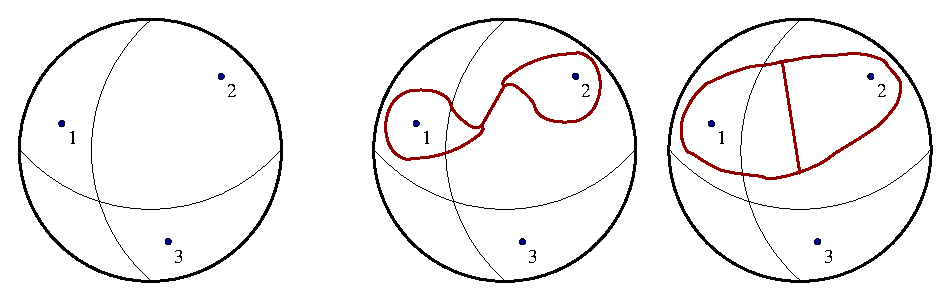
\includegraphics[width=\textwidth]{sfera3}
  \caption{A thrice-punctured sphere and two inequivalent
    deformation retracts.} 
  \label{fig:sphere-retracts}
\end{figure}
We look forward to refining this correspondence: let us introduce more
structure on the graph.
\begin{definition}
  \label{dfn:metric-ribbon-graphs}
  A metric ribbon graph is the data of ribbon graph $G$ equipped with
  a real positive number $\ell_\alpha$ for each edge $\alpha \in \Edges{G}$.
\end{definition}

We can give the topological Riemann surface $S(G)$ a complex structure
by means of a triangulation and an analytic atlas.

In the course of the construction of $S(G)$, two punctured disk have
been glued on the sides of an edge $\alpha \in \Edges{G}$: call them $\alpha^+$
and $\alpha^-$; they are not necessarily distinct.  Let $T_\alpha^+$ and $T_\alpha^-$
be the triangles delimited by $\alpha$ and the radii joining endpoints of
$\alpha$ with the puncture of $\alpha^\pm$. The collection $\{T_\alpha^\pm : \alpha \in
\Edges{G}\}$ is a triangulation of $S(G)$.

Define an atlas of $S(G)$:
\begin{itemize}
\item for any edge $\alpha \in \Edges{G}$, put $V_\alpha := (T_\alpha^+ \cup T_\alpha^-)^\circ$;
\item for any boundary component $\beta \in \Holes{G}$, put $V_\beta := \bigl(
  \bigcup_{\alpha} T_\alpha \bigr)^\circ$ for all $\alpha$ bounding $\beta$;
\item for any vertex $\gamma \in \Vertices{G}$, put $V_\gamma := \bigl( \bigcup_\alpha T_a^\pm
  \bigr)^\circ$ for all $\alpha$ incident to $\gamma$.
\end{itemize}
\begin{figure}[btp]
  %% Figura atlas.fig
  \centering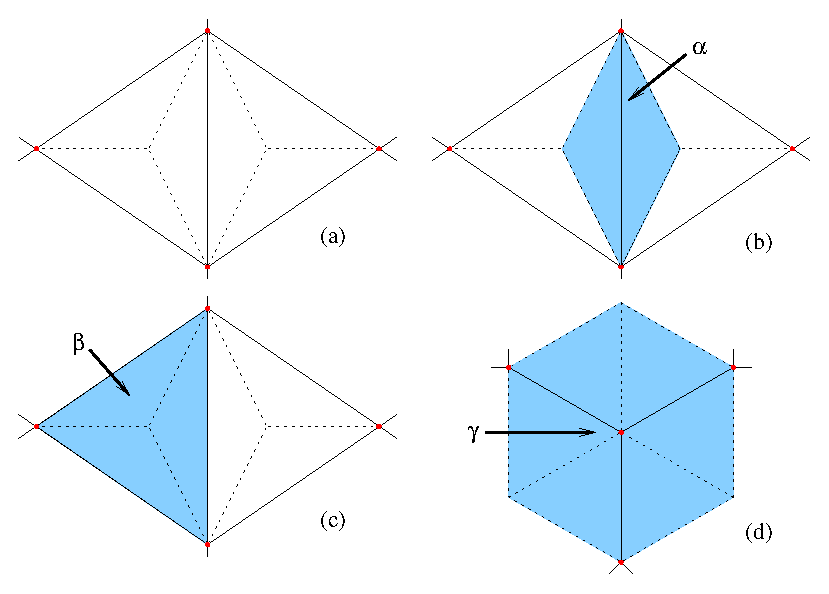
\includegraphics[width=\textwidth]{atlas}
  \caption{The open sets building an atlas of $S(G)$: (a) the
    triangulation built from a graph $G$: graph edges are drawn as
    solid lines, and edges of $T_\alpha^{\pm}$ are drawn as dotted lines; (b)
    the neighborhood $V_\alpha$ of an edge $\alpha$; (c) the neighborhood $V_\beta$
    of a hole $\beta$; (d) the neighborhood $V_\gamma$ of a vertex $\gamma$.}
  \label{fig:atlas}
\end{figure}

Define charts on the open sets $V$ (see Figure~\ref{fig:charts}):
\begin{itemize}
\item for any edge $\alpha$, pick a homeomorphism $f_\alpha: V_\alpha \to \{ z \in \setC
  : 0 < \Re z < \ell_\alpha \}$;
\item for any hole $\beta$, bounded by edges $\alpha_1$, $\alpha_2$ and $\alpha_3$,
  pick a homeomorphism $f_\beta: V_\beta \to \{ \abs{z} < \rho \}$, where $\rho =
  (\ell_{\alpha_1} + \ell_{\alpha_2} + \ell_{\alpha_3}) / 2\pi$.
\item for any vertex $\gamma$, pick a homeomorphism $f_\gamma: V_\gamma \to \setC$.
\end{itemize}
\begin{figure}[htbp]
  %% Figura charts.fig
  \centering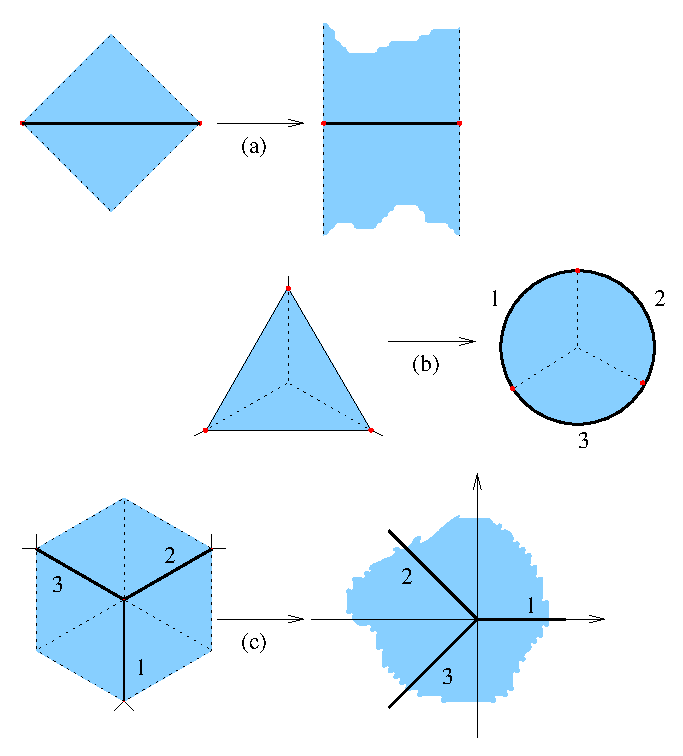
\includegraphics{charts}
  \caption{Local charts on the atlas: (a) any open set $V_\alpha$
    maps to a strip in the complex plane; (b) any open set $V_\beta$
    maps to a disk; (c) any open set $V_\gamma$ maps to the complex
    plane itself.}
  \label{fig:charts}
\end{figure}
These choices are subject to the condition that transition functions
satisfy the following:
\begin{itemize}
\item if $\alpha$ is an edge bounding the hole $\beta$, then $f_\beta \circ
  f_\alpha^{-1} = \exp (2\pi\I z / p_\beta)$ with $p_\beta := \sum_{\alpha \in \beta} \ell_\alpha$
  (\emph{perimeter} of the hole $\beta$);
\item if $\alpha$ is incident to a vertex $\gamma$, then $f_\gamma \circ f_\alpha^{-1} =
  c \cdot z^{2/(m+2)}$, up to a complex constant of modulus $1$, where
  $m$ is the valence of the vertex $\gamma$.
\end{itemize}

In the end, we have come upon a complex analytic structure on
$S(G)$, which depends on the perimeters $p_1, \ldots, p_n$ of holes $\beta_1,
\ldots, \beta_n$. By varying these (real positive) parameters, one can vary
the complex structure on $S(G)$; this will allow for a different
construction of the moduli space $\M_{g,n}$.


\subsection{The Jenkins-Strebel Theorem}
\label{sec:strebel}
A theorem proved independently by J.~A. Jenkins \cite{jenkins;annals}
and K.~Strebel \cite{strebel;quadratic-differentials;1983} provides
the key tool for the inverse route: the construction of ribbon graphs
from smooth complex curves.

\begin{definition}
  A quadratic differential $q$ on a Riemann surface $S$ is a
  (meromorphic) section of $(T^*S)\tp2$.
\end{definition}
The set of vectors in $T_zS$ on which $q$ takes real non-negative
values forms a real line in $T_zS$: therefore, they make up a
foliation $F = F_qS$ on $S \textbackslash{} \{\text{poles of $q$}\}$. The non-compact
leaves of $F$ together with zeroes of $q$ form the ``critical locus''
of $q$.  

The set of vectors ion $T_zS$ on which $q$ takes a purely imaginary
value form a perpendicular foliation $F^\perp$, whose leaves connect
either two distinct poles $x_i$ and $x_j$, or a pole $x_i$ and a zero
$v_j$.

Every quadratic differential $q$ induces a metric (away from the
critical locus) by $ds^2 = \abs{q(z)} \cdot \abs{\ud z}$.

\begin{theorem}[Jenkins, Strebel; {\cite[Theorem 23.2 and
    23.5]{strebel;quadratic-differentials;1983}}] For any complex
  analytic curve $S$ with $n$ marked points $x_1, \ldots, x_n$, and any
  assignment of real positive numbers $p_1, \ldots, p_n$, there exists one
  and only one quadratic differential $q$ such that:
  \begin{itemize}
  \item the only poles of $q$ occur at the marked points $x_1, \ldots, x_n$
    with second residue $p_1, ..., p_n$, that is, in a local
    coordinate $z_i$ near $x_i$ we have:
    \begin{equation*}
      q = p_i^2 (\d z_i / z_i) + \text{higher order terms};
    \end{equation*}
  \item the non-critical real trajectories of $F_q$ are simple closed
    circles around $x_i$.
  \end{itemize}
  Furthermore, $q$ has the following properties:
  \begin{itemize}
  \item every closed leaf circling around $x_i$ has length $p_i$ in the flat
    metric induced by $q$.
  \item the critical locus of $q$ is a graph $G$ embedded in $S$;
  \item the complement $S \textbackslash{} G$ of the critical locus is a collection
    of disks $\{D_i\}_{i=1,\ldots,n}$, each one centered at a pole $x_i$, and
    the projective class of the collection of radii of disks $\{D_i\}$
    equals the projective class $[p_1, \ldots, p_n]$.
  \end{itemize}
\end{theorem}
The critical graph $G$ inherits a structure of ribbon graph with
metric from the ambient surface $S$: the length of an edge $\alpha$ is the
one measured in the metric induced by the quadratic
differential. Furthermore, Jenkins-Strebel's theory states that $G$ has a
vertex of valence $k+2$ where $q$ has a zero of order $k$, therefore,
vertices of $G$ have valence $\geq3$.

Since the markings $x_1, \ldots, x_n$ are \emph{ordered}, $G$ has an
additional structure of \emph{numbered} graph, that is, it is endowed
with a bijection $h: \Holes{G} \to \{1, \ldots, n\}$. 


\subsection{Embedded ribbon graphs}
\label{sec:embedded-rg}




\subsection{Construction of the combinatorial analogues of $\T_{g,n}$
  and $\M_{g,n}$}
\label{sec:mgn-comb-construction}

Let $G$ be a metrized ribbon graph of genus $g$ with $n$ numbered
boundary components.  A topological cell $\Delta_G \subseteq \M_{g,n}$ is spanned
when varying the metric data $(\ell_\alpha)_{\alpha \in \Edges{G}}$; gluing these
cells one recovers the whole $\M_{g,n}$. We show here a quick
construction of $\M_{g,n}$ and $\T_{g,n}$, following
\cite{kontsevich;intersection-theory;1992} and
\cite{penner;teichmuller-theory}

\begin{definition}
  \label{dfn:strebel-graphs}
  Define a category $\Strebel[g,n]$, whose objects are metric numbered
  ribbon graphs with genus $g$ and $n$ holes, all whose vertices have
  valence $\geq3$ (call them ``JS graphs'', for short).  Morphisms
  $G \to G'$ are compositions of graph isomorphisms and contractions of
  an edge $\alpha \in \Edges{G}$.
\end{definition}

Call a set $X \subseteq \Edges{G}$ negligible whenever it is \emph{not} the
support of a non-trivial homological cycle.  Define
\begin{equation*}
  \label{eq:kontsevich-3}
  M(G) := \{ \ell: \Edges{G} \to \setR_{>0} | \text{the zero set of $\ell$ is negligible}\}.
\end{equation*}
It is a contravariant functor from the category of $\Strebel[g,n]$ of
metrized numbered ribbon graphs to the category of topological spaces:
if $G'$ is obtained from $G$ by contracting the edge $\alpha$, then
\begin{equation*}
  M(G') = \{ \ell \in M(G) | \ell_\alpha = 0 \}.
\end{equation*}
\begin{definition}
  The combinatorial moduli space of smooth algebraic curves is the
  direct limit of the functor $M$:
  \begin{equation*}
    \Mcomb_{g,n} := \varinjlim M(G),
  \end{equation*}
  with $G$ in the category $\Strebel[g,n]$ of metrized numbered ribbon
  graphs.
\end{definition}
\begin{remark}
  $\Mcomb_{g,n}$ is obtained by gluing orbicells $M(G)$ (quotient of
  a topological cell by $\Aut G$) alongside the boundary (if $G'$ is a
  contraction of $G$, then $M(G')$ is a face of $M(G)$). Therefore,
  $\Mcomb_{g,n}$ is a orbifold.
\end{remark}

It is easy to check that any $[G, \ell] \in \Mcomb_{g,n}$ has a unique
representative such that $\ell_\alpha > 0$ for all $\alpha \in \Edges{G}$.
The perimeter maps $p_\beta: \Mcomb_{g,n} \to \setR_{>0}$ are well-defined;
write $p_j$ for the perimeter of the $j$-th hole.

The construction of $\Mcomb_{g,n}$ can be done with slightly changed
rules: if we define a set $X \subseteq \Edges{G}$ to be negligible iff it does
not contain \emph{all} edges bounding a hole, then we can define a
contrafunctor $\overline{M}(G)$ and a topological space:
\begin{equation*}
  \label{eq:kontsevich-4}
  \Mbarcomb_{g,n} := \varinjlim \overline{M}(G).
\end{equation*}
$\Mbarcomb_{g,n}$ turns out to be a compactification of the orbifold
$\Mcomb_{g,n}$. 

\begin{theorem}[Harer, Mumford, Thurston;
  \cite{harer;cohomological-dimension, looijenga;cellular-decomposition}] 
  The Strebel construction defines morphisms
  \begin{equation*}
    \M_{g,n} \times \setR_{>0}^n \to \Mcomb_{g,n}, \qquad \Mbar_{g,n} \times
    \setR_{>0}^n \to \Mbarcomb_{g,n}.
  \end{equation*}
  The first of these is a homeomorphism and, more, an orbifold
  equivalence. The inverse map
  \begin{equation*}
    \Mcomb_{g,n} \to \M_{g,n} \times \setR_{>0}^n \to \setR_{>0}^n
  \end{equation*}
  is the perimeter map $\pi := (p_1, \ldots, p_n)$.  
\end{theorem}

For any given $p^\circ = (p_1^\circ, \ldots, p_n^\circ) \in \setR_{>0}^n$, the fiber
$\pi^{-1}(p^\circ)$ is isomorphic to $\M_{g,n}$, thus, $\pi$ induces a
triangulation of $\M_{g,n}$.

The cell $M(G)$ has real dimension $\card{\Edges{G}}$; therefore,
cells of maximal dimension are given by graphs with all vertices of
valence $3$. The union of these cells is a dense subset of
$\Mcomb_{g,n}$ with non-void interior.



\section{Arc-systems and their complexes}
\label{sec:arc-systems}

Harer \cite{harer;cohomological-dimension}, introduced the arc-systems
complex as a tool to reckon the (co)homology of the moduli space
$\M_{g,n}$.

Let $S_{g,n}$ be a topological compact oriented Riemann surface of
fixed genus $g$ with $n$ marked points $x_1, \ldots, x_n$.  Regard points
in the moduli space $\M_{g,n}$ as equivalence classes $(C,x,f)$ of a
complex curve $C$ with a marking $x:\{1,\ldots,n\}\to C$ and a homeomorphism
$f:C\to S_{g,n}$ with the reference surface (see
\csref{sec:alternate-Mgn}).

If $\alpha$ is any arc in $C$, denote by $[\alpha]$ its isotopy class rel~$\{x_1,
\ldots, x_n\}$.

\begin{definition}
  An arc-system $[\alpha_1, \ldots, \alpha_k]$ of rank $k$ is an isotopy class
  rel~$\{x_1, \ldots, x_n\}$ of $k$ properly imbedded arcs $\alpha_i : [0,1] \to C$
  such that:
  \begin{itemize}
  \item every $\alpha_i$ has its endpoints in the set $\{x_1, \ldots, x_n\}$;
  \item if $i \neq j$, then $\alpha_i$ meet $\alpha_j$ only at endpoints, if at all;
  \item no $\alpha_i$ is null-homotopic rel~$\{x_1, \ldots, x_n\}$;
  \item no $\alpha_i$ is homotopic rel~$\{x_1, \ldots, x_n\}$ to $\alpha_j$, for $i \neq
    j$;
  \end{itemize}
  An arc-system $[\alpha_1, \ldots, \alpha_k]$ is said to \emph{fill up} the curve
  $C$ iff all connected components of $C - \bigcup\{\alpha_i\} - \{x_1,\ldots x_n\}$ are
  either disks or punctured disks.
\end{definition}

Arc-systems may be organized into a semi-simplicial complex.
\begin{definition}
  $X$ is the semi-simplicial complex having a simplex $\langle\alpha_1, \ldots, \alpha_k\rangle$
  for every rank $k$ arc-system $[\alpha_1, \ldots \alpha_k]$, with the proviso that
  $\langle\beta_1, \ldots, \beta_l\rangle$ is a face of $\langle\alpha_1, \ldots, \alpha_k\rangle$ iff $\{ [\beta_1], \ldots, [\beta_l]
  \} \subset \{ [\alpha_1], \ldots, [\alpha_k] \}$.
  
  $X_\infty$ is the subcomplex of all those simplices $\langle\alpha_1, \ldots, \alpha_k\rangle$
  that do not fill up the surface $S$.
\end{definition}

Let $\Delta^{n-1}$ be the $(n-1)$-dimensional geometric simplex.
\begin{theorem}[Harer, {\cite[Theorem
  1.3]{harer;cohomological-dimension}}]
There exists a $\Gamma_{g,n}$-equivariant homeomorphism $\Phi: \T_{g,n} \times
\Delta^{n-1} \to X \setminus X_\infty$.
\end{theorem}

Let $X^\circ$, $X_\infty^\circ$ be the first barycentric subdivisions of $X$
and $X_\infty$, respectively.

\begin{definition}
  Let $Y^\circ$ be the collection of simplices in $X^\circ$ having no face in
  $X_\infty^\circ$; equivalently, $\sigma_\bullet \in Y^\circ$ iff every vertex of $\sigma_\bullet$
  lies in $X^\circ \setminus X_\infty^\circ$.  $Y^\circ$ is a full subcomplex of $X^\circ$.
\end{definition}




%%% Local Variables: 
%%% mode: latex
%%% TeX-master: "index"
%%% x-symbol-8bits: nil
%%% End: 


